% Canonical SpectraNet architecture diagram (hand-drawn, drawio source at
% paper/SpectraNet-Architecture.drawio; export at paper/SpectraNet-Architecture-crop.pdf,
% deployed to paper/figures/architecture.pdf). The earlier matplotlib generator
% (paper/scripts/make_architecture_figure.py) is deprecated and should not be re-run.
\begin{figure}[ht]
\centering
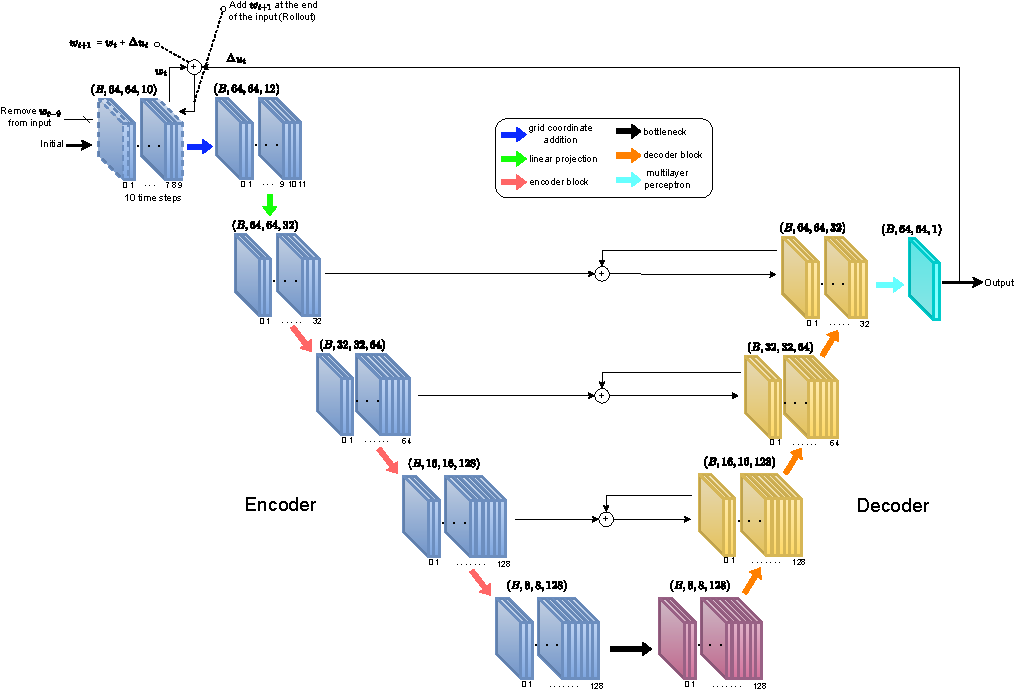
\includegraphics[width=0.58\textwidth]{figures/architecture.pdf}
\caption{\textbf{SpectraNet architecture.} Input $(B,64,64,10)$ + $(x,y)$-grid
(\emph{blue}) is lifted to $w{=}32$ channels (\emph{green}); a three-level encoder
(\emph{red}) at truncations $M_\ell\!\in\!\{12,6,3\}$ feeds a single-block bottleneck
(\emph{black}, $M_3{=}1$); a mirrored decoder (\emph{orange}) upsamples with additive
skips (\emph{$\oplus$}); a two-layer $1{\times}1$ MLP head (\emph{cyan}, hidden $4w$,
GeLU) emits the residual $\Delta_\theta$, summed with $\omega_t$ (\emph{curved $+$})
to recover $\widehat{\omega}_{t+1}$ (\Cref{thm:approx-stab}).}
\label{fig:architecture}
\end{figure}
